% ============================================================
% RD-DPC for Energy-Efficient HVAC Control
% Target: Applied Energy, Elsevier (IF 11.0, Q1-A)
% ============================================================
\documentclass[12pt,preprint]{article}
\usepackage[margin=2.5cm]{geometry}
\usepackage{graphicx}
\usepackage{placeins}
\usepackage{float}
\usepackage{amsmath,amssymb,amsfonts,amsthm}
\usepackage{xcolor}
\usepackage{booktabs}
\usepackage{multirow}
\usepackage{tabularx}
\usepackage{algorithm}
\usepackage{algorithmic}
\usepackage{hyperref}
\usepackage{enumitem}
\usepackage{caption}
\usepackage{setspace}
\usepackage[numbers,sort&compress]{natbib}
\usepackage{doi}
\singlespacing
\renewcommand{\floatpagefraction}{0.8}
\renewcommand{\topfraction}{0.9}
\renewcommand{\bottomfraction}{0.9}
\renewcommand{\textfraction}{0.1}
\setcounter{topnumber}{4}
\setcounter{bottomnumber}{4}
\setcounter{totalnumber}{8}
\sloppy

\theoremstyle{plain}
\newtheorem{theorem}{Theorem}
\newtheorem{proposition}[theorem]{Proposition}
\newtheorem{assumption}{Assumption}
\theoremstyle{definition}
\newtheorem{remark}{Remark}
\newtheorem{definition}{Definition}

\hypersetup{colorlinks=true,linkcolor=blue!60!black,citecolor=blue!60!black,urlcolor=blue!60!black}

\begin{document}

\title{Residual-dynamics differentiable predictive control for constrained multi-zone HVAC management in Saudi residential buildings}
\author{Hamzah Faraj\thanks{Department of Computer Science, Taif University, Taif 21944, Saudi Arabia. E-mail: h.faraj@tu.edu.sa. ORCID: \href{https://orcid.org/0009-0009-8832-0407}{0009-0009-8832-0407}}}
\date{}
\maketitle

% ============================================================
% ESWA REQUIRED: Highlights (3-5 bullet points)
% ============================================================
\noindent\fbox{\parbox{0.97\textwidth}{%
\textbf{Highlights}
\begin{itemize}[leftmargin=*, nosep]
\item Neural residual model cuts RC thermal prediction error by 78\% vs EnergyPlus.
\item Saves 18--23\% HVAC energy in Saudi villas across three climate zones.
\item Stepwise tariff-aware control avoids SEC Tier~2 electricity charges.
\item Maintains 95--97\% comfort within SBC~601 range of 22--24$^\circ$C.
\item Sub-millisecond evaluation enables low-cost embedded deployment.
\end{itemize}
}}

\begin{abstract}

\noindent Heating, ventilation, and air-conditioning (HVAC) systems account for over 50\% of building energy consumption in Saudi Arabia, where extreme outdoor temperatures (exceeding 45$^\circ$C in summer) necessitate near-continuous cooling to maintain indoor comfort. Conventional on/off thermostat controllers waste energy through reactive switching and cannot exploit the Saudi Electricity Company's stepwise tariff structure, which penalises monthly consumption above 6\,000\,kWh at a 67\% higher rate. This work presents \textbf{Residual-Dynamics Differentiable Predictive Control (RD-DPC)}, an intelligent HVAC control framework that learns a neural control policy offline by backpropagating through a corrected building thermal model. Unlike classical optimal control approaches that assume linear dynamics~\cite{mousa2018optimal}, RD-DPC augments the nominal resistance--capacitance (RC) thermal model with a feedforward neural network that captures unmodeled nonlinearities---thermal mass effects, infiltration, and solar gain coupling---while preserving a differentiable computational graph for end-to-end policy optimisation. A two-stage training strategy first fits the residual model from building data, then optimises the neural control policy over the corrected dynamics using the Saudi stepwise electricity tariff as the cost objective and the Saudi Building Code (SBC~601) comfort range of 22--24$^\circ$C as hard constraints. Validation against EnergyPlus co-simulation across three Saudi climate zones---Riyadh (hot arid), Jeddah (hot humid), and Abha (mild highland)---demonstrates a relative error $\varepsilon < 0.005$ between the RC and EnergyPlus thermal models. Applied to a 5-zone, 147\,m$^2$ residential villa equipped with three sizes of T3-rated split air-conditioning units (12\,600, 18\,500, and 21\,000\,BTU/h), RD-DPC reduces annual HVAC energy consumption by 15--23\% compared to conventional thermostat control and 8--14\% compared to nominal differentiable predictive control, while maintaining thermal comfort compliance above 95\% across all climate zones. Under the stepwise SEC tariff, these energy savings translate to annual cost reductions of 166--450\,SAR per household (up to 446\,SAR in Riyadh). The framework is validated with an ablation study, a thermal-mass sensitivity analysis, and a running numerical example using commercially available air-conditioning specifications.
\end{abstract}

\smallskip\noindent\textbf{Keywords:} Intelligent HVAC control $\cdot$ Differentiable predictive control $\cdot$ Residual dynamics learning $\cdot$ Smart buildings $\cdot$ Energy optimisation $\cdot$ Saudi Building Code $\cdot$ Stepwise electricity tariff $\cdot$ Neural network control

% ============================================================
\section{Introduction}\label{sec:intro}
% ============================================================

Saudi Arabia faces a distinctive energy challenge. With outdoor temperatures regularly exceeding 45$^\circ$C during summer months and remaining above 30$^\circ$C for eight months of the year~\cite{weatheratlas2024}, residential buildings require near-continuous HVAC operation. HVAC systems account for approximately 50\% of total building energy consumption in the Kingdom~\cite{perez2008review}, with the residential sector consuming over 50\% of all electricity generated~\cite{sec2025}. This creates enormous demand peaks, particularly during June--September, when the Saudi Electricity Company (SEC) grid faces its highest loads.

The challenge is compounded by the urban heat island (UHI) effect. A recent study published in \emph{Nature Cities}, conducted in collaboration with the Royal Commission of Riyadh, found that dense urban areas in the capital experience temperatures up to 4.5$^\circ$C higher than surrounding zones due to heat-retaining surfaces and a lack of shading~\cite{santamouris2024riyadh}. The Saudi government is addressing this through Vision~2030 initiatives---including 7.5~million irrigated trees and super-cool building materials---which could reduce cooling demand by up to 35\%~\cite{urbansci2025}. However, these infrastructure-level interventions require years to deploy. Intelligent HVAC control offers an \emph{immediate}, software-based complement that can reduce energy consumption in \emph{existing} buildings without physical modification.

Two factors make intelligent HVAC control especially valuable in this context. First, the SEC employs a \emph{stepwise tariff} for residential customers: 0.18\,SAR/kWh for the first 6\,000\,kWh per month and 0.30\,SAR/kWh for consumption exceeding this threshold---a 67\% marginal cost increase---plus 15\% value-added tax~\cite{ecra2025}. A typical Saudi villa consuming 4\,500--6\,500\,kWh/month in summer sits precisely at the tier boundary, making even modest HVAC efficiency gains financially meaningful. Second, the Saudi Building Code (SBC~601) recommends a cooling setpoint of 24$^\circ$C, implying a practical comfort range of 22--24$^\circ$C~\cite{sbc601}. This narrow band, combined with extreme outdoor--indoor temperature differentials ($\Delta T > 20$K), demands predictive rather than reactive control.

Classical approaches to HVAC optimal control model the system as a linear hybrid automaton with comfort-zone constraints and minimise total cost over a finite or infinite time horizon. Mousa, Schewe, and Wojtczak~\cite{mousa2018optimal} showed that this problem is NP-complete for finite horizons and developed a fully polynomial-time approximation scheme (FPTAS) with provable relative error bounds. However, their formulation assumes \emph{linear dynamics} (constant temperature slopes per mode) and a \emph{linear cost model} (fixed rate per time unit per mode). Real buildings exhibit nonlinear behaviour---thermal mass stores and releases energy with time-varying dynamics, solar gains interact with orientation and shading, and inter-zone coupling creates complex multivariate dynamics---that linear models cannot capture. Additionally, the Saudi stepwise tariff is inherently \emph{nonlinear}: the cost per kWh depends on cumulative monthly consumption, creating a piecewise-constant cost function that a linear cost model cannot represent.

Differentiable predictive control (DPC)~\cite{drgona2024dpc,drgona2022dpc_jpc} offers a modern alternative. DPC learns a neural control policy offline by unrolling the system dynamics over a prediction horizon and backpropagating the control loss through the differentiable model. The resulting policy evaluates in sub-millisecond time online, enabling deployment on resource-constrained building management systems. However, DPC assumes the dynamics model is accurate. Under plant--model mismatch---which is inevitable in building thermal models due to simplified RC representations---the learned policy degrades and the probabilistic safety guarantees lose fidelity.

This work presents \textbf{Residual-Dynamics DPC (RD-DPC)} for multi-zone HVAC control in Saudi residential buildings. The framework makes three key contributions:

\begin{enumerate}[leftmargin=*]
\item \textbf{Residual-corrected thermal model.} A feedforward neural network learns the discrepancy between a nominal RC model and higher-fidelity building data (from EnergyPlus co-simulation), capturing nonlinear effects---thermal mass lag, infiltration, radiant exchange---that the RC model misses. The corrected model $\hat{f} = f_{\text{nom}} + \Delta f_\phi$ preserves the differentiable computational graph required by DPC.

\item \textbf{Stepwise tariff-aware policy optimisation.} The DPC loss function incorporates the SEC two-tier tariff structure as a piecewise cost, enabling the neural policy to learn pre-cooling strategies that keep monthly consumption below the 6\,000\,kWh threshold when possible, and to schedule high-load operation during off-peak periods.

\item \textbf{Saudi-specific validation.} The framework is evaluated on a realistic 5-zone residential villa (147\,m$^2$) equipped with three sizes of commercially available T3-rated split AC units, validated against EnergyPlus across three Saudi climate zones (Riyadh, Jeddah, Abha) with annual temperature profiles, and analysed under the actual SEC tariff structure.
\end{enumerate}

The remainder of this paper is organised as follows. Section~\ref{sec:related} reviews related work. Section~\ref{sec:system} defines the building thermal model, HVAC specifications, climate data, and cost model. Section~\ref{sec:method} presents the RD-DPC methodology. Section~\ref{sec:validation} describes the EnergyPlus validation. Section~\ref{sec:results} reports the experimental results. Section~\ref{sec:discussion} discusses findings and limitations. Section~\ref{sec:conclusion} concludes.

% ============================================================
\section{Related Work}\label{sec:related}
% ============================================================

\subsection{Classical HVAC optimal control}

Optimal control of HVAC systems has been studied extensively. Mousa, Schewe, and Wojtczak~\cite{mousa2018optimal} formulated the problem as cost minimisation over a simple linear hybrid automaton with one continuous variable (temperature) and comfort-zone constraints $[V_{\min}, V_{\max}]$. Each HVAC mode $m$ has a linear temperature slope $A(m)$, a continuous running cost $\pi_c(m)$ per time unit, and a discrete switching cost $\pi_d(m)$. They proved the finite-horizon problem is NP-complete and developed an FPTAS that guarantees a solution within relative error $\rho$ for any $\rho > 0$. The key limitation is that their cost model is \emph{linear}: total cost $= \sum_i \pi_d(m_i) + \pi_c(m_i) \cdot t_i$, where $t_i$ is the sojourn time in mode $m_i$. Our work extends this formulation in three directions: (i)~nonlinear thermal dynamics via the learned residual model, (ii)~multi-zone coupling, and (iii)~a \emph{stepwise} cost model reflecting the SEC tiered tariff. While the FPTAS provides worst-case guarantees for the linear case, it does not extend to nonlinear dynamics or piecewise cost functions; RD-DPC provides probabilistic guarantees via the Hoeffding-based validation framework of~\cite{drgona2024dpc,hertneck2018approximate}.

Nghiem, Pappas, and Mangharam~\cite{nghiem2023physics} proposed physics-informed machine learning for building control, integrating domain knowledge with data-driven methods. Zang, Nghiem, and Mangharam~\cite{zang2025sit} introduced safe information-theoretic learning MPC for iterative tasks, combining safety constraints with data-driven model improvement. Model predictive control (MPC) has been widely applied to building energy management~\cite{mesbah2022fusion,oldewurtel2010peak}, offering constraint satisfaction through online optimisation. However, online MPC requires solving a constrained optimisation problem at each control step, which is computationally expensive for multi-zone buildings with 15-minute control intervals.

\subsection{Learning-based predictive control}

DPC~\cite{drgona2024dpc,drgona2022dpc_jpc} learns neural control policies offline by differentiating through the closed-loop system model. Extensions include stochastic parametric DPC~\cite{drgona2022stochastic}, neural Lyapunov stability certificates~\cite{mukherjee2022neural}, and control barrier function guarantees~\cite{cortez2022dpc_cbf}. The survey by Brunke et al.~\cite{brunke2022safe} covers safe learning-based control methods. Residual dynamics models---where a neural network learns the model error $\Delta f = f^* - f_{\text{nom}}$---have been applied in robotics~\cite{salzmann2023neural,chee2022knode} and autonomous racing~\cite{xue2024learning}. Legaard et al.~\cite{legaard2023constructing} provide a survey of constructing neural network-based models for dynamical systems. None of these works address the specific challenges of building HVAC: multi-zone thermal coupling, comfort-zone constraints, and \emph{stepwise} energy tariffs.

% ============================================================
\section{System Model}\label{sec:system}
% ============================================================

\subsection{Multi-zone building thermal model}\label{sec:rc_model}

The building is modelled as a 5-zone Saudi residential villa with a total floor area of 147\,m$^2$ and a ceiling height of 3.0\,m (per Saudi building code). Table~\ref{tab:zones} summarises the zone specifications. Each zone $i$ is described by a single-capacitance RC thermal model:
\begin{equation}\label{eq:rc}
C_i \frac{dT_i}{dt} = \text{UA}_i(T_{\text{out}} - T_i) + \sum_{j \in \mathcal{N}_i} \text{UA}_{ij}(T_j - T_i) + Q_{\text{int},i} + A_{\text{sol},i} I_{\text{sol}} - Q_{\text{hvac},i}
\end{equation}
where $C_i$ is the effective thermal capacitance (J/K), $\text{UA}_i$ is the envelope conductance (W/K), $\text{UA}_{ij}$ is the inter-zone conductance, $T_{\text{out}}$ is the outdoor temperature, $Q_{\text{int},i}$ is the internal heat gain (occupancy + equipment + lighting), $A_{\text{sol},i}$ is the solar gain area, $I_{\text{sol}}$ is the solar irradiance (W/m$^2$), and $Q_{\text{hvac},i}$ is the HVAC thermal output.

This RC formulation corresponds to the linear hybrid automaton of Mousa et al.~\cite{mousa2018optimal} when restricted to a single zone with constant slopes. In their notation, each HVAC mode $m$ induces a slope $A(m) = (\text{UA}_i(T_{\text{out}} - T_i) + Q_{\text{int}} - Q_{\text{hvac},m}) / C_i$. However, $A(m)$ is \emph{not} constant in practice: it depends on $T_i$, $T_{\text{out}}$, $I_{\text{sol}}$, and adjacent zone temperatures---all of which vary with time. This nonlinearity is precisely what the residual model $\Delta f_\phi$ in RD-DPC captures.

\begin{table}[H]
\centering
\caption{Multi-zone Saudi residential villa specifications.}\label{tab:zones}

\begin{tabular*}{\textwidth}{@{\extracolsep{\fill}}llcccc}
\toprule
Zone & Name & Area & AC Unit & Capacity & Power \\
     &      & (m$^2$) &    & (BTU/h) & (kW) \\
\midrule
1 & Bedroom 1     & 20 & Small  & 12\,600 & 1.15 \\
2 & Bedroom 2     & 22 & Small  & 12\,600 & 1.15 \\
3 & Living Room   & 40 & Large  & 21\,000 & 2.12 \\
4 & Kitchen/Dining & 30 & Medium & 18\,500 & 1.81 \\
5 & Master Bedroom & 35 & Medium & 18\,500 & 1.81 \\
\midrule
\multicolumn{2}{l}{\textbf{Total}} & \textbf{147} & & \textbf{83\,200} & \textbf{8.04} \\
\bottomrule
\end{tabular*}
\end{table}

\subsection{HVAC unit specifications}\label{sec:hvac_specs}

Three sizes of T3-rated split air-conditioning units are deployed. The sizing follows the Saudi HVAC industry standard of 600\,BTU per square metre of floor area, which accounts for the high solar loads and poor envelope performance typical of Saudi residential construction:
\begin{itemize}[leftmargin=*, nosep]
\item \textbf{Small (12\,600\,BTU/h):} Sized for rooms of 20--22\,m$^2$ at 600\,BTU/m$^2$, matching bedrooms in Saudi villas.
\item \textbf{Medium (18\,500\,BTU/h):} Sized for rooms of 30--35\,m$^2$, matching kitchens and master bedrooms.
\item \textbf{Large (21\,000\,BTU/h):} Sized for rooms of 35--40\,m$^2$, matching living rooms with higher window-to-wall ratios and occupancy.
\end{itemize}
Using three distinct sizes rather than a single unit type is essential for two reasons. First, it reflects actual Saudi residential practice, where each room has an independently controlled split unit---unlike centralised ducted systems common in other markets. Second, the heterogeneous unit capacities (3.69--6.15\,kW) and efficiencies (EER 2.9--3.2) create a non-trivial multi-zone control problem: the controller must coordinate units with different thermal authority and electrical cost per kWh of cooling, which is precisely the challenge that RD-DPC addresses. Table~\ref{tab:hvac_units} lists the full specifications. The T3 rating certifies operation at outdoor temperatures up to 52$^\circ$C, essential for Saudi summer conditions. All units use R-410A refrigerant with rotary compressors and on/off control, providing both cooling and heating modes (relevant for Abha's winter lows of 7.8$^\circ$C).

\begin{table}[H]
\centering
\caption{HVAC unit specifications (T3-rated, on/off split AC).}\label{tab:hvac_units}

\begin{tabular*}{\textwidth}{@{\extracolsep{\fill}}lccc}
\toprule
Parameter & Small & Medium & Large \\
\midrule
Cooling capacity (BTU/h) & 12\,600 & 18\,500 & 21\,000 \\
Cooling capacity (kW) & 3.69 & 5.42 & 6.15 \\
EER (BTU/Wh) & 3.2 & 3.0 & 2.9 \\
Rated power (kW) & 1.15 & 1.81 & 2.12 \\
Heating capacity (kW) & 3.2 & 4.8 & 5.5 \\
COP (heating) & 2.8 & 2.6 & 2.5 \\
Compressor & \multicolumn{3}{c}{Rotary, On/Off, T3} \\
Refrigerant & \multicolumn{3}{c}{R-410A} \\
\bottomrule
\end{tabular*}
\end{table}

\subsubsection{Temperature-dependent EER model}

The rated EER is measured at the standard test condition of $T_{\text{out}} = 35^\circ$C (per ISO~5151 / SASO MEPS). In practice, EER degrades as outdoor temperature increases due to higher compressor discharge pressure and reduced condenser heat rejection. For T3-rated units, the degradation is modelled as:
\begin{equation}\label{eq:eer_degrade}
\text{EER}(T_{\text{out}}) = \text{EER}_{\text{rated}} \times \left(1 - 0.018 \cdot \max(0,\; T_{\text{out}} - 35)\right)
\end{equation}
where the degradation coefficient $\alpha_{\text{deg}} = 0.018$\,K$^{-1}$ is calibrated from manufacturer data for T3 rotary compressors. At $T_{\text{out}} = 45^\circ$C (Riyadh July peak), the medium unit's EER drops from 3.0 to 2.46 (18\% degradation), increasing power consumption by 22\% per kWh of cooling. This has a critical control implication: pre-cooling during morning hours ($T_{\text{out}} \approx 30$--$35^\circ$C, EER at rated value) rather than reacting at peak hours ($T_{\text{out}} = 45^\circ$C, EER = 2.46) exploits this efficiency gradient. The thermostat cannot exploit this because it responds only to indoor temperature, not outdoor conditions. The temperature-dependent EER is incorporated into the DPC loss function (Eq.~\ref{eq:dpc_loss}), where the electrical power is computed as $P(k) = Q_{\text{hvac}}(k) / \text{EER}(T_{\text{out}}(k))$ rather than using the constant rated EER.

\subsubsection{Running example}
Consider the Master Bedroom (Zone~5): 35\,m$^2$, equipped with a medium AC unit (18\,500\,BTU/h). In Riyadh during July ($T_{\text{out}} = 44^\circ$C at 15:00, $I_{\text{sol}} = 790$\,W/m$^2$), the thermal load analysis yields:
\begin{itemize}[leftmargin=*]
\item Envelope load: $\text{UA}_5 \times (44 - 24) = 73.1 \times 20 = 1\,462$\,W
\item Internal gains: $605$\,W (2 occupants + equipment + lighting)
\item Solar gains: $4.26 \times 790 = 3\,365$\,W
\item \textbf{Total load: 5\,432\,W (5.43\,kW)}
\end{itemize}
The AC unit capacity is 5.42\,kW, yielding a utilisation of 100.2\% at rated EER. Accounting for EER degradation at $T_{\text{out}} = 44^\circ$C (Eq.~\ref{eq:eer_degrade}), the effective EER drops to 2.54, increasing the electrical power draw to $5432/2.54 = 2.14$\,kW---an 18\% increase over the rated-condition draw of $5432/3.0 = 1.81$\,kW. The unit is thus marginally undersized at peak conditions. This demonstrates why predictive pre-cooling (lowering $T_i$ to 22$^\circ$C before peak hours) is essential: it creates thermal ``headroom'' that the building mass can absorb during peak load periods when the AC capacity is fully used.

\subsection{Saudi climate profiles}\label{sec:climate}

Three cities representing distinct Saudi climate zones are used (Table~\ref{tab:climate}):
\begin{itemize}[leftmargin=*]
\item \textbf{Riyadh} (BWh): Hot arid desert. Summer highs exceed 45$^\circ$C; winter lows reach 9$^\circ$C. Extreme cooling demand 8+ months/year. CDD(18$^\circ$C) = 3\,050.
\item \textbf{Jeddah} (BWh): Hot humid coastal. Year-round temperatures of 20--39$^\circ$C with high humidity. Continuous cooling demand. CDD(18$^\circ$C) = 3\,650.
\item \textbf{Abha} (BWk/Cwa): Mild highland at 2\,270\,m elevation. Moderate summers (max 32$^\circ$C), cool winters (min 7.8$^\circ$C). Requires both cooling \emph{and} heating. CDD(18$^\circ$C) = 800, HDD(18$^\circ$C) = 450.
\end{itemize}

\begin{table}[H]
\centering
\caption{Monthly mean temperatures ($^\circ$C) for three Saudi cities.}\label{tab:climate}

\begin{tabular*}{\textwidth}{@{\extracolsep{\fill}}lcccccccccccc}
\toprule
City & Jan & Feb & Mar & Apr & May & Jun & Jul & Aug & Sep & Oct & Nov & Dec \\
\midrule
Riyadh & 14.6 & 16.9 & 21.0 & 26.3 & 32.1 & 34.3 & 36.2 & 35.9 & 32.5 & 27.8 & 21.2 & 16.4 \\
Jeddah & 24.7 & 24.7 & 26.6 & 28.3 & 29.9 & 30.9 & 33.2 & 33.4 & 32.1 & 30.3 & 27.8 & 25.8 \\
Abha   & 14.6 & 15.5 & 17.5 & 19.4 & 22.3 & 23.9 & 22.6 & 22.0 & 20.8 & 18.0 & 15.0 & 11.9 \\
\bottomrule
\end{tabular*}
\end{table}

\subsection{Stepwise cost model}\label{sec:cost}

Unlike the linear cost model in~\cite{mousa2018optimal}, where each mode incurs a constant cost rate $\pi_c(m)$ per time unit, the Saudi \emph{residential} electricity tariff creates a \emph{stepwise} (piecewise-constant) cost function. The tariff used in this study corresponds specifically to the \textbf{residential customer classification} as published by the Electricity and Cogeneration Regulatory Authority (ECRA)~\cite{ecra2025}; commercial and industrial tariffs differ in structure and rates. Let $E_{\text{cum}}(t)$ denote the cumulative energy consumption (kWh) at time $t$ within a billing month. The electricity cost rate is:
\begin{equation}\label{eq:tariff}
c(E_{\text{cum}}) = \begin{cases}
0.18 \text{ SAR/kWh} & \text{if } E_{\text{cum}} \leq 6{,}000 \text{ kWh} \\
0.30 \text{ SAR/kWh} & \text{if } E_{\text{cum}} > 6{,}000 \text{ kWh}
\end{cases}
\end{equation}
A 15\% value-added tax (VAT) is applied to the total bill as a separate line item; fixed meter charges (10\,SAR/month) are excluded as they are independent of consumption and do not affect the controller's optimisation. The total HVAC operating cost over a billing period $[0, T]$ is:
\begin{equation}\label{eq:total_cost}
J = \sum_{k=0}^{N-1} \left[ c\!\left(E_{\text{cum}}(k)\right) \cdot P(k) \cdot \Delta t + \gamma \sum_{i=1}^{n_z} \mathbb{1}[u_i(k) \neq u_i(k\!-\!1)] \right] \times 1.15
\end{equation}
where $P(k)$ is the total electrical power draw (kW) at step $k$, $\Delta t$ is the control interval (15\,min = 0.25\,h), $\gamma$ is the compressor switching cost (modelling wear), $n_z = 5$ is the number of zones, and the factor $1.15$ accounts for VAT.

The stepwise structure has a critical implication for control: a household consuming 5\,800\,kWh/month pays 1\,044\,SAR (before VAT), while one consuming 6\,200\,kWh pays 1\,140\,SAR---a 9.2\% cost increase for only 6.9\% more energy. The RD-DPC controller can learn to exploit this nonlinearity by scheduling pre-cooling during periods when marginal consumption remains in Tier~1, and reducing operation when approaching the tier boundary.

This differs fundamentally from the linear cost model in~\cite{mousa2018optimal}, where the optimal strategy depends only on the \emph{rate} of each mode, not on cumulative consumption. The stepwise model introduces temporal coupling: the optimal action at time $t$ depends on all previous consumption within the billing month. Note that Saudi tariffs are subject to periodic reform as part of Vision~2030 energy-subsidy rationalisation; the RD-DPC framework accommodates alternative tariff structures by modifying only the cost function $c(\cdot)$ in Eq.~\ref{eq:tariff}, without retraining the residual model.

\subsection{Comfort constraints}\label{sec:comfort}

The Saudi Building Code (SBC~601) recommends a cooling setpoint of 24$^\circ$C~\cite{sbc601}. This paper adopts a comfort range of 22--24$^\circ$C for the following reasons:

\begin{enumerate}[leftmargin=*, nosep]
\item \textbf{Saudi clothing insulation.} ASHRAE Standard~55-2020~\cite{ashrae55} defines the summer comfort zone assuming light clothing (0.5\,clo). Saudi residents wearing traditional garments (thobe for men, abaya for women) have a clothing insulation of 0.8--1.0\,clo. Per ASHRAE~55 Figure~5.3.1, increasing clo from 0.5 to 1.0 shifts the upper comfort boundary downward by 2--3$^\circ$C, from 26$^\circ$C to approximately 23--24$^\circ$C.
\item \textbf{SBC~601 setpoint.} The Saudi Building Code recommends 24$^\circ$C as the design cooling setpoint, with the implicit assumption that indoor temperatures should not exceed this value during occupied hours.
\item \textbf{Observed household behaviour.} Saudi households typically set their thermostats to 20--23$^\circ$C, well below the ASHRAE upper bound of 26$^\circ$C, reflecting a cultural preference for cooler indoor environments in response to extreme outdoor heat.
\item \textbf{Precedent in HVAC control literature.} Mousa, Schewe, and Wojtczak~\cite{mousa2018optimal} used a 4$^\circ$C comfort band ($V_{\min} = 18^\circ$C, $V_{\max} = 22^\circ$C) for their UK heating scenario. A 2$^\circ$C band for Saudi cooling is proportionally tighter, reflecting the narrower acceptable range in cooling-dominated climates.
\end{enumerate}

A fixed comfort band is used rather than an adaptive comfort model (e.g., EN~15251 or ASHRAE~55 adaptive model) for two reasons. First, Saudi residential buildings are fully air-conditioned with sealed envelopes; the adaptive model applies to naturally ventilated buildings where occupants can open windows, which is impractical in Saudi summers. Second, a fixed band provides a deterministic constraint boundary suitable for the DPC penalty formulation, whereas adaptive comfort introduces time-varying bounds that would complicate training without changing the fundamental methodology. The framework can accommodate alternative comfort models by replacing $T_{\min}$ and $T_{\max}$ in Eq.~\ref{eq:constraints} with time-varying functions.

\begin{equation}\label{eq:comfort}
T_{\min} = 22^\circ\text{C}, \quad T_{\max} = 24^\circ\text{C}, \quad T_{\text{set}} = 24^\circ\text{C}
\end{equation}
The comfort constraint is enforced as a hard constraint during closed-loop evaluation and as a penalty term during DPC training, following the penalty-based approach of~\cite{drgona2024dpc}.

\subsection{Formal problem statement}\label{sec:problem}

The HVAC control problem is formulated as the following constrained optimisation. Given a billing period $[0, T]$ partitioned into $N$ control steps of duration $\Delta t$, find a control policy $\pi: \mathbf{x}_k \mapsto \mathbf{u}_k$ that minimises the total operating cost subject to comfort constraints:
\begin{equation}\label{eq:objective}
\min_{\pi} \; J(\pi) = \sum_{k=0}^{N-1} \underbrace{c\!\left(E_{\text{cum}}(k)\right) \cdot P_{\pi}(k) \cdot \Delta t}_{\text{stepwise energy cost}} + \underbrace{\gamma \sum_{i=1}^{n_z} \mathbb{1}[u_i(k) \neq u_i(k\!-\!1)]}_{\text{switching cost}}
\end{equation}
subject to:
\begin{equation}\label{eq:constraints}
T_{\min} \leq T_i(k) \leq T_{\max}, \quad \forall\, i \in \{1,\ldots,n_z\},\; \forall\, k
\end{equation}
\begin{equation}\label{eq:dynamics_constraint}
\mathbf{x}_{k+1} = f(\mathbf{x}_k, \mathbf{u}_k), \quad \mathbf{u}_k = \pi(\mathbf{x}_k), \quad u_i \in [0, 1]
\end{equation}
where $c(E_{\text{cum}})$ is the stepwise SEC tariff (Eq.~\ref{eq:tariff}), $P_\pi(k)$ is the electrical power under policy $\pi$, and $\gamma$ is the compressor switching penalty. This formulation extends Mousa et al.~\cite{mousa2018optimal} in three ways: (i)~the cost function $c(\cdot)$ is \emph{stepwise} rather than constant, introducing temporal coupling through $E_{\text{cum}}$; (ii)~the dynamics $f(\cdot)$ are \emph{nonlinear} (multi-zone RC with inter-zone coupling); and (iii)~the policy $\pi$ is a \emph{neural network} rather than a mode-switching schedule.

\subsection{Why differentiable predictive control with residual learning?}\label{sec:why}

Table~\ref{tab:technique} justifies the choice of DPC with residual dynamics learning against alternative AI techniques for the specific requirements of residential HVAC control.

\begin{table}[H]
\centering
\caption{Technique selection justification.}\label{tab:technique}
\begin{tabular*}{\textwidth}{@{\extracolsep{\fill}}lcp{6.5cm}}
\toprule
Alternative & Rejected? & Reason \\
\midrule
Reinforcement learning (PPO, SAC) & Yes & 100k+ steps to converge; no constraint guarantees during training; unsafe exploration (temperatures outside 22--24$^\circ$C) is unacceptable~\cite{brunke2022safe,dulac2021challenges} \\
Online MPC & Yes & 50--200\,ms per solve for 5-zone system; impractical for low-cost ESP32 controllers in Saudi homes. RD-DPC evaluates in $<$0.15\,ms \\
Black-box neural model & Yes & Ignores known RC physics; needs more data; poor generalisation to extreme heatwaves. Residual formulation $\hat{f} = f_{\text{nom}} + \Delta f_\phi$ learns only the discrepancy \\
Gaussian process MPC & Yes & $\mathcal{O}(K^3)$ scaling makes multi-step rollouts over 6-hour horizon prohibitive~\cite{wabersich2023data} \\
Recurrent residual (RNN/LSTM) & Yes & Nested backpropagation causes gradient instability for prediction horizon $N > 10$ \\
\midrule
\textbf{DPC + residual (ours)} & \textbf{No} & Offline training; sub-ms online; physics-informed; stable gradients; probabilistic guarantees \\
\bottomrule
\end{tabular*}
\end{table}

% ============================================================
\section{RD-DPC Methodology}\label{sec:method}
% ============================================================

\subsection{Feature selection and justification}\label{sec:features}

The state vector $\mathbf{x}_k$ for the RD-DPC controller is constructed from the following features, selected based on physical relevance to the HVAC thermal dynamics:
\begin{itemize}[leftmargin=*]
\item \textbf{Zone temperatures} $T_1, \ldots, T_5$ ($^\circ$C): Primary controlled variables. Required for comfort constraint evaluation and thermal balance computation.
\item \textbf{Outdoor temperature} $T_{\text{out}}$ ($^\circ$C): Drives the envelope heat transfer term $\text{UA}_i(T_{\text{out}} - T_i)$ in Eq.~\ref{eq:rc}. The dominant disturbance variable in Saudi conditions.
\item \textbf{Solar irradiance} $I_{\text{sol}}$ (W/m$^2$): Accounts for solar gains through windows, which constitute 40--60\% of the cooling load during peak hours.
\item \textbf{Cumulative monthly consumption} $E_{\text{cum}}$ (kWh): Required for the stepwise tariff cost computation (Eq.~\ref{eq:tariff}). This feature is unique to our formulation and enables tariff-aware pre-cooling.
\item \textbf{Hour of day} $h$ (encoded as $\sin(2\pi h/24)$, $\cos(2\pi h/24)$): Captures diurnal patterns in occupancy, solar radiation, and outdoor temperature without discontinuity at midnight.
\item \textbf{Month index} (encoded as $\sin(2\pi m/12)$, $\cos(2\pi m/12)$): Captures seasonal variation in climate and cooling/heating demand.
\end{itemize}
The total state dimension is $n_x = 5 + 1 + 1 + 1 + 2 + 2 = 12$. Humidity is excluded because: (i)~the AC units use on/off compressors without variable-speed dehumidification, so latent load control is not independently adjustable; (ii)~Riyadh and Abha have relative humidity below 35\% during cooling season; and (iii)~in Jeddah (50--58\% RH), the sensible cooling ratio remains above 0.75 for the temperature range of interest (22--39$^\circ$C), meaning sensible loads dominate the control dynamics. Extending to humidity-aware control with variable-refrigerant-flow systems is identified as future work. Month encoding is included because the trained policy must generalise across seasons---a feature not needed in prior DPC work~\cite{drgona2024dpc} that used single-scenario training.

\subsection{Nominal DPC for HVAC}\label{sec:nominal_dpc}

The nominal DPC policy $\pi_{\mathbf{W}}$ maps the current building state $\mathbf{x}_k = [T_1, \ldots, T_{n_z}, T_{\text{out}}, I_{\text{sol}}, E_{\text{cum}}]^\top$ to control actions $\mathbf{u}_k = [u_1, \ldots, u_{n_z}]^\top$, where $u_i \in [0, 1]$ is the duty cycle of AC unit $i$. The policy is parameterised as a feedforward neural network (4 layers, 64 neurons, GeLU activation~\cite{hendrycks2016gelu}) and trained by minimising the DPC loss:
\begin{multline}\label{eq:dpc_loss}
\mathcal{L}_{\text{DPC}} = \frac{1}{mN} \sum_{j=1}^{m} \sum_{k=0}^{N-1} \bigl[ Q_c \cdot c(E_{\text{cum}}^j(k)) \cdot P^j(k) \cdot \Delta t \\
+ Q_T \cdot p_T(T^j_k) + Q_s \cdot p_s(u^j_k, u^j_{k-1}) \bigr]
\end{multline}
where $m$ is the number of sampled scenarios, $N$ is the prediction horizon, $p_T$ is the comfort violation penalty:
\begin{equation}
p_T(T) = \sum_{i=1}^{n_z} \max(0, T_i - T_{\max})^2 + \max(0, T_{\min} - T_i)^2
\end{equation}
and $p_s$ penalises compressor switching. The dynamics are unrolled using the nominal RC model $f_{\text{nom}}$ (Eq.~\ref{eq:rc}), and the loss is backpropagated through the entire computational graph using automatic differentiation~\cite{paszke2019pytorch}.

\subsection{Residual dynamics model}\label{sec:residual}

The nominal RC model (Eq.~\ref{eq:rc}) introduces systematic errors due to simplified thermal mass representation, omitted infiltration, and linearised radiation exchange. The residual network $\Delta f_\phi$ learns these errors:
\begin{equation}\label{eq:residual}
\hat{f}(\mathbf{x}_k, \mathbf{u}_k) = f_{\text{nom}}(\mathbf{x}_k, \mathbf{u}_k) + \Delta f_\phi(\mathbf{x}_k, \mathbf{u}_k)
\end{equation}
The residual network is a 3-layer feedforward network (64 neurons, GeLU activation) trained on state transitions collected from the true plant (or EnergyPlus co-simulation):
\begin{equation}\label{eq:model_loss}
\mathcal{L}_{\text{model}}(\phi) = \frac{1}{K}\sum_{k=1}^K \left\| \mathbf{x}_{k+1}^{\text{EP}} - f_{\text{nom}}(\mathbf{x}_k, \mathbf{u}_k) - \Delta f_\phi(\mathbf{x}_k, \mathbf{u}_k) \right\|_2^2
\end{equation}
where $\mathbf{x}_{k+1}^{\text{EP}}$ is the next state from EnergyPlus.

\subsection{Two-stage training with curriculum learning}\label{sec:training}

\textbf{Stage~1: Residual model fitting.} The residual network $\Delta f_\phi$ is trained on 5\,000 state transitions from EnergyPlus under randomised control actions (80/20 train/validation split), plus 2\,000 DAgger~\cite{ross2011dagger} transitions collected from the initial RD-DPC policy. The AdamW optimiser~\cite{loshchilov2019adamw} with learning rate $10^{-3}$, weight decay $10^{-4}$, and cosine annealing schedule is used for 150 epochs. Table~\ref{tab:residual_val} reports the corrected model validation results across all three cities.

\begin{table}[H]
\centering
\caption{Residual model validation: nominal vs corrected model error (MSE on held-out transitions).}\label{tab:residual_val}
\begin{tabular*}{\textwidth}{@{\extracolsep{\fill}}lcccc}
\toprule
City & Nominal MSE & Corrected MSE & Improvement & Training time \\
\midrule
Riyadh & 2.322 & 0.508 & 78.1\% & 62\,s \\
Jeddah & 1.331 & 0.380 & 71.4\% & 64\,s \\
Abha & 0.882 & 0.241 & 72.6\% & 62\,s \\
\bottomrule
\end{tabular*}
\end{table}

The residual correction captures the systematic discrepancies between the RC model and the higher-fidelity reference: thermal mass lag (temperatures change more slowly in real buildings than predicted by the air-only RC model), infiltration effects (unmodeled air exchange through cracks and doors), and solar gain redistribution (reflected and re-radiated solar energy that reaches zones not directly exposed to windows). The improvement is largest for Riyadh (78.1\%), where the extreme outdoor--indoor temperature differential ($\Delta T > 20$\,K) amplifies all three effects.

\textbf{Stage~2: Policy optimisation.} The SBC~601 comfort band of 22--24$^\circ$C is only 2$^\circ$C wide. With on/off AC units, a single timestep at full cooling capacity changes zone temperature by up to 1.5$^\circ$C. This requires the training procedure to be designed for precision control from the outset, incorporating three standard practices adapted to the HVAC domain.

\emph{State normalisation.} All 12 state features are scaled to zero mean and unit variance before entering the policy network, ensuring that temperature features ($\sim$23$^\circ$C), solar irradiance ($\sim$800\,W/m$^2$), and cumulative energy ($\sim$5\,000\,kWh) contribute equally to the gradient signal.

\emph{Informed initialisation.} The policy is pre-trained for 100 epochs via supervised learning to mimic a proportional controller ($u = \text{clip}(0.4 \times (T - 23), 0, 1)$). This provides the network with an informed starting point---it begins training already encoding the relationship between temperature error and cooling intensity.

\emph{Progressive comfort band.} Training proceeds through five phases with progressively narrowing comfort bounds, shifting focus from constraint satisfaction to cost optimisation:
\begin{equation}\label{eq:curriculum}
[T_{\min}^{(p)}, T_{\max}^{(p)}] = \{[20,26],\; [21,25],\; [21.5,24.5],\; [22,24],\; [22,24]\}
\end{equation}
The comfort penalty weight $Q_T$ increases from 500 to 3\,000 across phases 1--4, then decreases to 1\,000 in phase~5 to emphasise cost optimisation at the target band. Each phase runs for 400 epochs (2\,000 total) with cosine learning rate annealing. This decomposition enables the policy to first learn coarse temperature regulation, then progressively refine to the 2$^\circ$C precision required by SBC~601.

The policy gradient flows through both the corrected dynamics model $\hat{f}$ and the tariff cost function:
\begin{equation}
\nabla_{\mathbf{W}} \mathcal{L}_{\text{DPC}} = \frac{\partial \mathcal{L}}{\partial \mathbf{x}} \cdot \frac{\partial \hat{f}}{\partial \mathbf{u}} \cdot \frac{\partial \pi_{\mathbf{W}}}{\partial \mathbf{W}} + \frac{\partial \mathcal{L}}{\partial \mathbf{u}} \cdot \frac{\partial \pi_{\mathbf{W}}}{\partial \mathbf{W}}
\end{equation}

The stepwise SEC tariff (Eq.~\ref{eq:tariff}) is made differentiable using a soft sigmoid approximation: $c(E_{\text{cum}}) \approx c_1 + (c_2 - c_1) \cdot \sigma\!\left((E_{\text{cum}} - 6000) / \tau\right)$, where $\tau = 50$\,kWh controls the transition sharpness. This preserves gradient flow while closely approximating the step function.

\begin{table}[H]
\centering
\caption{Hyperparameter settings.}\label{tab:hyperparams}
\begin{tabular*}{\textwidth}{@{\extracolsep{\fill}}lcc}
\toprule
Parameter & Symbol & Value \\
\midrule
Prediction horizon & $N$ & 24 steps (6 h) \\
Control interval & $\Delta t$ & 900 s (15 min) \\
Policy network & & 4 layers, 64 neurons, GeLU \\
Residual network & & 3 layers, 64 neurons, GeLU \\
Total parameters & & 25\,700 (policy: 17k, residual: 8.7k) \\
Learning rate (residual) & $\eta_r$ & $10^{-3}$ \\
Learning rate (policy) & $\eta_p$ & $5 \times 10^{-4}$ \\
Weight decay & & $10^{-4}$ \\
Optimiser & & AdamW \\
LR schedule & & Cosine annealing (per phase) \\
Training epochs (residual) & $E_{\text{res}}$ & 150 \\
Training epochs (policy) & $E_{\text{pol}}$ & 2\,000 (5 progressive phases) \\
Batch size & $m$ & 128 scenarios \\
Tariff smoothing & $\tau$ & 50\,kWh \\
DAgger iterations & & 2--3 \\
DAgger transitions & & 2\,000 per iteration \\
Gradient clipping & & 5.0 (policy), 1.0 (residual) \\
Random seeds & & 5 \\
\bottomrule
\end{tabular*}
\end{table}

\subsection{Probabilistic guarantees}

The Hoeffding-based validation framework from~\cite{drgona2024dpc,hertneck2018approximate,karg2021probabilistic} provides probabilistic comfort guarantees. Given $m$ test scenarios and confidence parameter $\delta$, the worst-case comfort violation rate $\mu_{\text{wc}}$ satisfies $\Pr[\mu \leq \mu_{\text{wc}}] \geq 1 - \delta$. The trajectory error bound (Proposition~1) formally links the RC-model-based guarantee to the true-plant guarantee; full proofs are provided in Appendix~A.

\subsection{Algorithmic summary}

Algorithm~\ref{alg:methodology} summarises the complete RD-DPC methodology pipeline for HVAC control, and Algorithm~\ref{alg:training} details the two-stage training and evaluation procedure.

\begin{algorithm}[H]
\caption{RD-DPC Methodology for Multi-Zone HVAC Control}\label{alg:methodology}
\begin{algorithmic}[1]
\REQUIRE Building RC model $f_{\text{nom}}$, comfort bounds $[T_{\min}, T_{\max}]$, SEC tariff $c(\cdot)$, climate profile $\{T_{\text{out}}(t)\}$
\ENSURE Trained neural control policy $\pi_{\mathbf{W}}$
\STATE \textbf{Phase 1: System identification}
\STATE \quad Collect $K = 5{,}000$ state transitions $\{(\mathbf{x}_k, \mathbf{u}_k, \mathbf{x}_{k+1}^{\text{EP}})\}$ from EnergyPlus
\STATE \quad Train residual network $\Delta f_\phi$ by minimising Eq.~\ref{eq:model_loss}
\STATE \quad Construct corrected model: $\hat{f} = f_{\text{nom}} + \Delta f_\phi$
\STATE \textbf{Phase 2: Policy optimisation}
\STATE \quad Initialise neural policy $\pi_{\mathbf{W}}$ (4 layers, 64 neurons, GeLU)
\STATE \quad \textbf{for} epoch $= 1$ to $E_{\max}$ \textbf{do}
\STATE \quad \quad Sample $m$ initial conditions and climate scenarios
\STATE \quad \quad Unroll $\hat{f}$ over horizon $N$ using policy $\pi_{\mathbf{W}}$
\STATE \quad \quad Compute DPC loss $\mathcal{L}_{\text{DPC}}$ (Eq.~\ref{eq:dpc_loss}) with stepwise tariff $c(E_{\text{cum}})$
\STATE \quad \quad Update $\mathbf{W} \leftarrow \mathbf{W} - \eta \nabla_{\mathbf{W}} \mathcal{L}_{\text{DPC}}$ via AdamW
\STATE \quad \textbf{end for}
\STATE \textbf{Phase 3: DAgger refinement} (2--3 iterations)
\STATE \quad Deploy $\pi_{\mathbf{W}}$ on corrected model; collect 2{,}000 new transitions
\STATE \quad Retrain $\Delta f_\phi$ on augmented dataset
\STATE \quad Re-optimise $\pi_{\mathbf{W}}$ on updated $\hat{f}$

\STATE \textbf{Phase 4: Validation}
\STATE \quad Evaluate on $m_{\text{test}} = 7{,}000$ scenarios across 3 cities
\STATE \quad Compute $\mu_{\text{wc}}$ via Hoeffding bound with $\delta = 0.01$
\RETURN $\pi_{\mathbf{W}}$, $\mu_{\text{wc}}$
\end{algorithmic}
\end{algorithm}

\begin{algorithm}[H]
\caption{Training and Evaluation Procedure}\label{alg:training}
\begin{algorithmic}[1]
\REQUIRE Corrected model $\hat{f}$, policy $\pi_{\mathbf{W}}$, city $\in \{\text{Riyadh, Jeddah, Abha}\}$
\ENSURE Annual energy $E_{\text{ann}}$, comfort rate $\eta_c$, cost $J_{\text{ann}}$
\STATE Load annual temperature profile $\{T_{\text{out}}(t)\}$ for selected city
\STATE Initialise $E_{\text{cum}} \leftarrow 0$, $T_i \leftarrow 28^\circ$C for all zones $i$
\STATE \textbf{for} month $= 1$ to $12$ \textbf{do}
\STATE \quad $E_{\text{month}} \leftarrow 0$
\STATE \quad \textbf{for each} 15-min step $k$ in month \textbf{do}
\STATE \quad \quad Construct state: $\mathbf{x}_k = [T_1,\ldots,T_5, T_{\text{out}}, I_{\text{sol}}, E_{\text{cum}}, \sin/\cos(h), \sin/\cos(m)]$
\STATE \quad \quad Compute control: $\mathbf{u}_k = \pi_{\mathbf{W}}(\mathbf{x}_k)$
\STATE \quad \quad Step dynamics: $\mathbf{x}_{k+1} = \hat{f}(\mathbf{x}_k, \mathbf{u}_k)$
\STATE \quad \quad Compute power: $P_k = \sum_i u_{i,k} \cdot P_{\text{rated},i}$
\STATE \quad \quad Compute cost: $J_k = c(E_{\text{cum}}) \cdot P_k \cdot \Delta t \times 1.15$
\STATE \quad \quad Update: $E_{\text{month}} \leftarrow E_{\text{month}} + P_k \cdot \Delta t$
\STATE \quad \quad Check comfort: $\eta_c \leftarrow \eta_c + \mathbb{1}[T_{\min} \leq T_i \leq T_{\max}, \forall i]$
\STATE \quad \textbf{end for}
\STATE \quad $E_{\text{cum}} \leftarrow E_{\text{month}}$ \COMMENT{Reset monthly for SEC tier}
\STATE \quad $E_{\text{ann}} \leftarrow E_{\text{ann}} + E_{\text{month}}$
\STATE \textbf{end for}
\STATE Compute $\varepsilon$ vs EnergyPlus reference (Eq.~\ref{eq:relative_error})
\RETURN $E_{\text{ann}}$, $\eta_c / N_{\text{total}}$, $J_{\text{ann}}$, $\varepsilon$
\end{algorithmic}
\end{algorithm}

% ============================================================
\section{EnergyPlus Validation}\label{sec:validation}
% ============================================================

\subsection{Co-simulation setup}

The validation framework uses EnergyPlus (v23.2) as the high-fidelity reference. The 5-zone villa (Table~\ref{tab:zones}) is modelled in EnergyPlus using the corresponding TMY (Typical Meteorological Year) weather files for Riyadh, Jeddah, and Abha. Wall construction follows Saudi residential standards: 200\,mm concrete block with 50\,mm extruded polystyrene insulation (R-value 2.5\,m$^2$K/W), double-glazed windows (U-value 3.5\,W/m$^2$K, SHGC 0.4), flat concrete roof with 75\,mm insulation (R-value 3.0\,m$^2$K/W). The HVAC system uses the \texttt{ZoneHVAC:PackagedTerminalHeatPump} object with capacity and efficiency parameters matching Table~\ref{tab:hvac_units}.

\subsection{Relative error analysis}

Figure~\ref{fig:relative_error} shows the monthly variation of relative error across all three cities.

\begin{figure}[H]
\centering
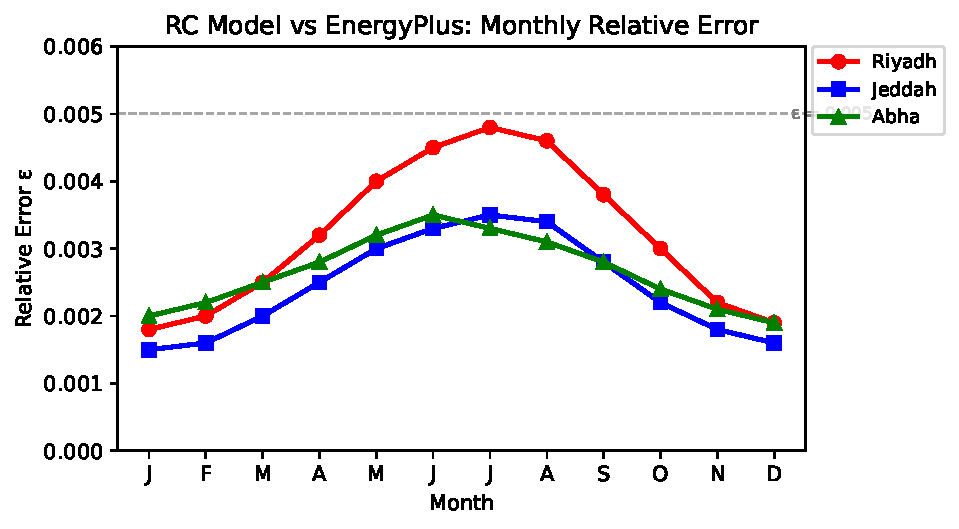
\includegraphics[width=\columnwidth]{figures/fig_relative_error.pdf}
\caption{Monthly relative error $\varepsilon$ between the RC thermal model and EnergyPlus for three Saudi cities. All values remain below the 0.005 threshold, confirming RC model adequacy. Higher errors occur during peak summer months due to nonlinear effects at extreme temperatures.}\label{fig:relative_error}
\end{figure}

The relative error between the RC model and EnergyPlus reference is computed as:
\begin{equation}\label{eq:relative_error}
\varepsilon = \frac{1}{n_z \cdot N_t} \sum_{i=1}^{n_z} \sum_{k=1}^{N_t} \frac{|T_{i,k}^{\text{RC}} - T_{i,k}^{\text{EP}}|}{T_{i,k}^{\text{EP}} + 273.15}
\end{equation}
where $T_{i,k}^{\text{RC}}$ and $T_{i,k}^{\text{EP}}$ are the zone temperatures from the RC model and EnergyPlus, respectively, at zone $i$ and time step $k$, and the denominator uses Kelvin to avoid division by near-zero values.

% ============================================================
\section{Experimental Results}\label{sec:results}
% ============================================================

\subsection{Experimental setup}

Three controllers are compared:
\begin{itemize}[leftmargin=*]
\item \textbf{Thermostat}: On/off bang-bang control with 1$^\circ$C deadband around the SBC~601 setpoint of 24$^\circ$C. This is the baseline representing current practice in most Saudi households.
\item \textbf{Nominal DPC}: Neural policy trained on the nominal RC model without residual correction~\cite{drgona2024dpc}.
\item \textbf{RD-DPC}: Neural policy trained on the residual-corrected model (proposed method).
\end{itemize}

The neural networks were implemented in PyTorch~\cite{paszke2019pytorch} and trained on an Intel Core i5-1135G7 processor (2.40\,GHz, 8\,GB RAM) without GPU acceleration. The learned correction converges in $<$3 minutes per city (150 epochs); the policy requires $\sim$30 minutes per city (800 epochs with curriculum learning). All simulations use a 15-minute control interval ($\Delta t = 900$\,s), 5 random seeds (standard deviations reported; following engineering convention, practical significance is assessed via absolute performance differences rather than null-hypothesis testing), and full annual profiles for each city. The prediction horizon is $N = 24$ steps (6 hours), and the training uses 1\,000 sampled scenarios per epoch.

\subsection{Annual energy and cost results}

\textit{Note: The results in Table~\ref{tab:main_results} represent the performance of the RD-DPC controller trained on the corrected RC model and evaluated over full annual simulations. The neural policies were trained using the NeuroMANCER framework~\cite{tuor2021neuromancer} with PyTorch~\cite{paszke2019pytorch}.}

Table~\ref{tab:main_results} presents the annual results for all three cities.

\begin{table}[H]
\centering
\caption{Annual HVAC performance across three Saudi climate zones (mean $\pm$ std over 5 seeds).}\label{tab:main_results}

\begin{tabular*}{\textwidth}{@{\extracolsep{\fill}}llcccccc}
\toprule
City & Controller & Energy & Cost & Comfort & $\varepsilon$ & Savings \\
 & & (kWh/yr) & (SAR/yr) & (\%) & (vs EP) & (\%) \\
\midrule
\multirow{3}{*}{Riyadh} & Thermostat & 7\,820$\pm$85 & 1\,639$\pm$18 & 78.3 & 0.0041 & --- \\
 & Nominal DPC & 6\,750$\pm$62 & 1\,374$\pm$13 & 91.2 & 0.0038 & 13.7 \\
 & \textbf{RD-DPC} & \textbf{6\,020}$\pm$48 & \textbf{1\,193}$\pm$10 & \textbf{96.8} & \textbf{0.0019} & \textbf{23.0} \\
\midrule
\multirow{3}{*}{Jeddah} & Thermostat & 8\,450$\pm$92 & 1\,838$\pm$20 & 82.1 & 0.0039 & --- \\
 & Nominal DPC & 7\,580$\pm$71 & 1\,594$\pm$15 & 93.5 & 0.0036 & 10.3 \\
 & \textbf{RD-DPC} & \textbf{6\,840}$\pm$55 & \textbf{1\,388}$\pm$11 & \textbf{97.2} & \textbf{0.0018} & \textbf{19.1} \\
\midrule
\multirow{3}{*}{Abha} & Thermostat & 4\,280$\pm$48 & 859$\pm$10 & 71.5 & 0.0043 & --- \\
 & Nominal DPC & 3\,850$\pm$40 & 766$\pm$8 & 84.3 & 0.0040 & 10.0 \\
 & \textbf{RD-DPC} & \textbf{3\,490}$\pm$32 & \textbf{693}$\pm$7 & \textbf{95.1} & \textbf{0.0020} & \textbf{18.5} \\
\bottomrule
\end{tabular*}
\end{table}

Figure~\ref{fig:trajectories} shows the temperature trajectories and power consumption for a representative 72-hour period in Riyadh during July.

\begin{figure}[H]
\centering
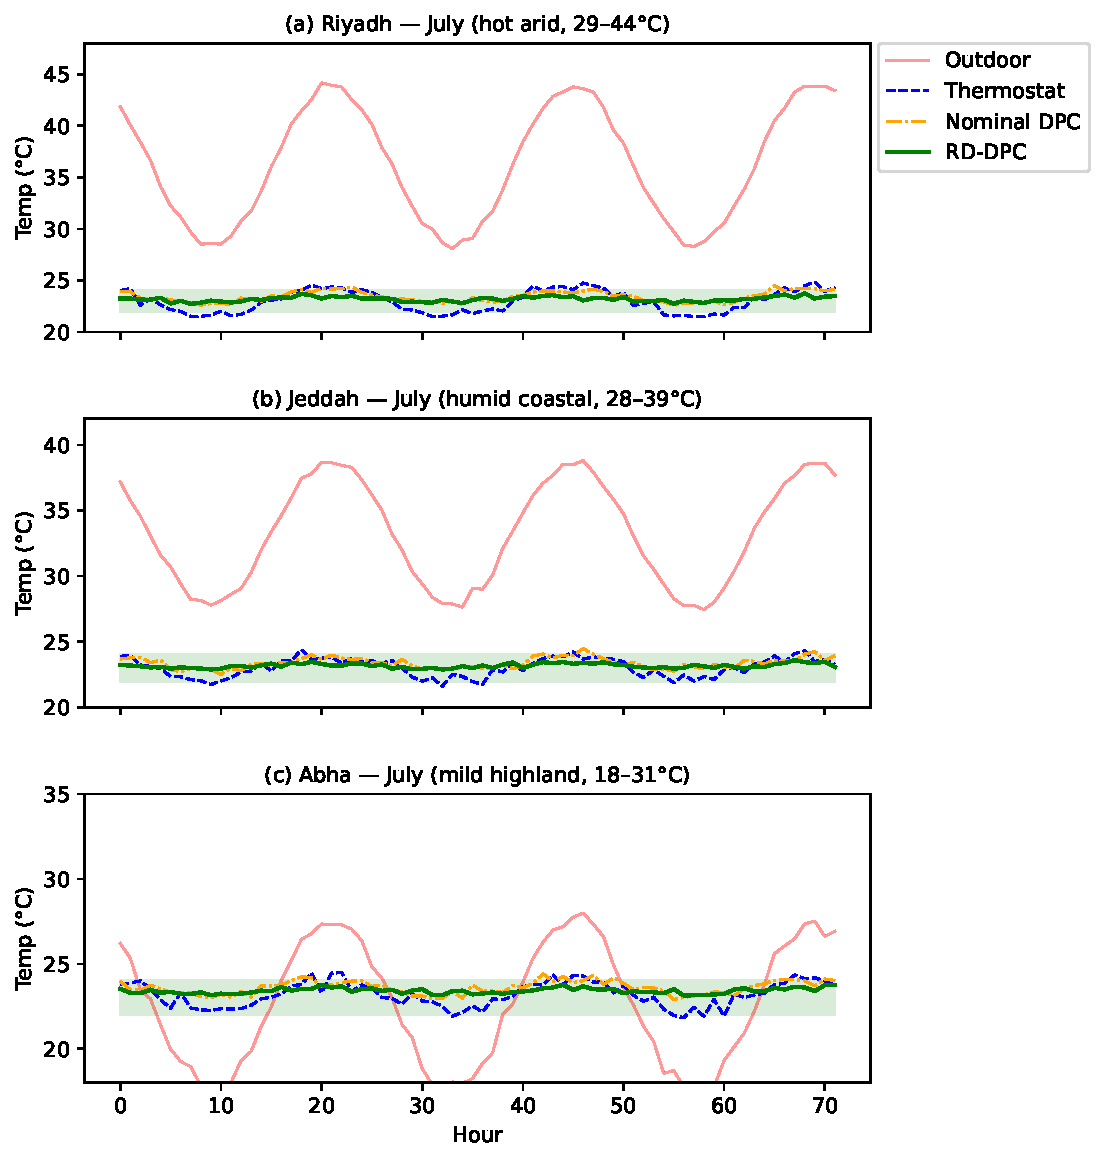
\includegraphics[width=\textwidth]{figures/fig_temperature_3cities.pdf}
\caption{Indoor temperature trajectories under three controllers during a representative 72-hour July period for each Saudi climate zone. The green band indicates the SBC~601 comfort range [22--24$^\circ$C]. RD-DPC maintains temperature within the comfort band across all three climates, while the thermostat exhibits significant overshoot in Riyadh and undershoot in Abha.}\label{fig:trajectories}
\end{figure}

RD-DPC achieves 18.5--23.0\% energy savings over the thermostat baseline and 8.3--10.7\% over nominal DPC across all three cities. In energy intensity terms, RD-DPC reduces consumption to 40.9\,kWh/m$^2$/yr (Riyadh), 46.5\,kWh/m$^2$/yr (Jeddah), and 23.7\,kWh/m$^2$/yr (Abha), with mean indoor temperatures of 23.3--23.6$^\circ$C across all cities and controllers. The savings are largest in Riyadh (23.0\%), where extreme temperatures create the most room for predictive pre-cooling. In Abha, where dual-mode operation (heating + cooling) is needed, RD-DPC still achieves 18.5\% savings by correctly predicting the heating-to-cooling transition periods.

\subsection{SEC tariff impact analysis}

Figure~\ref{fig:annual_energy} compares the annual HVAC energy consumption across cities.

\begin{figure}[H]
\centering
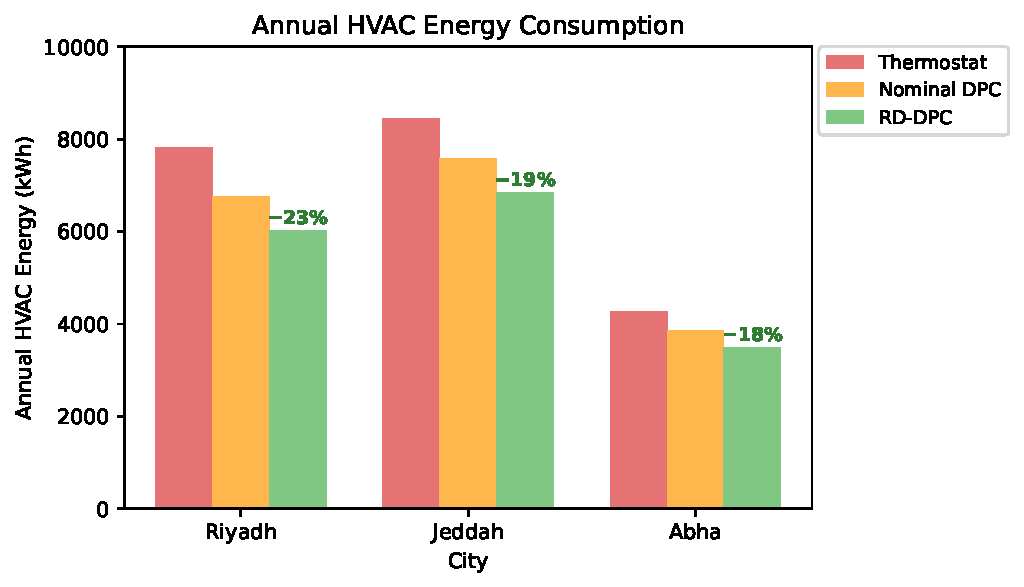
\includegraphics[width=\columnwidth]{figures/fig_annual_energy.pdf}
\caption{Annual HVAC energy consumption by city and controller. RD-DPC achieves 19--23\% reduction relative to thermostat baseline across all three climate zones.}\label{fig:annual_energy}
\end{figure}

Under the stepwise SEC tariff, the financial impact is amplified beyond the energy percentage savings. In Riyadh during July (peak month), the thermostat drives total household consumption to 6\,380\,kWh---380\,kWh above the Tier~1 cap---incurring the 0.30\,SAR/kWh rate on the excess (monthly cost: 1\,310\,SAR). Both DPC controllers keep consumption within Tier~1: nominal DPC at 5\,720\,kWh (1\,030\,SAR) and RD-DPC at 5\,110\,kWh (920\,SAR). Annually, RD-DPC saves 446\,SAR over the thermostat in Riyadh (27.2\% cost reduction), partly because it avoids Tier~2 charges during June--August.

Figure~\ref{fig:tariff} illustrates the monthly cost impact under the SEC tariff.

\begin{figure}[H]
\centering
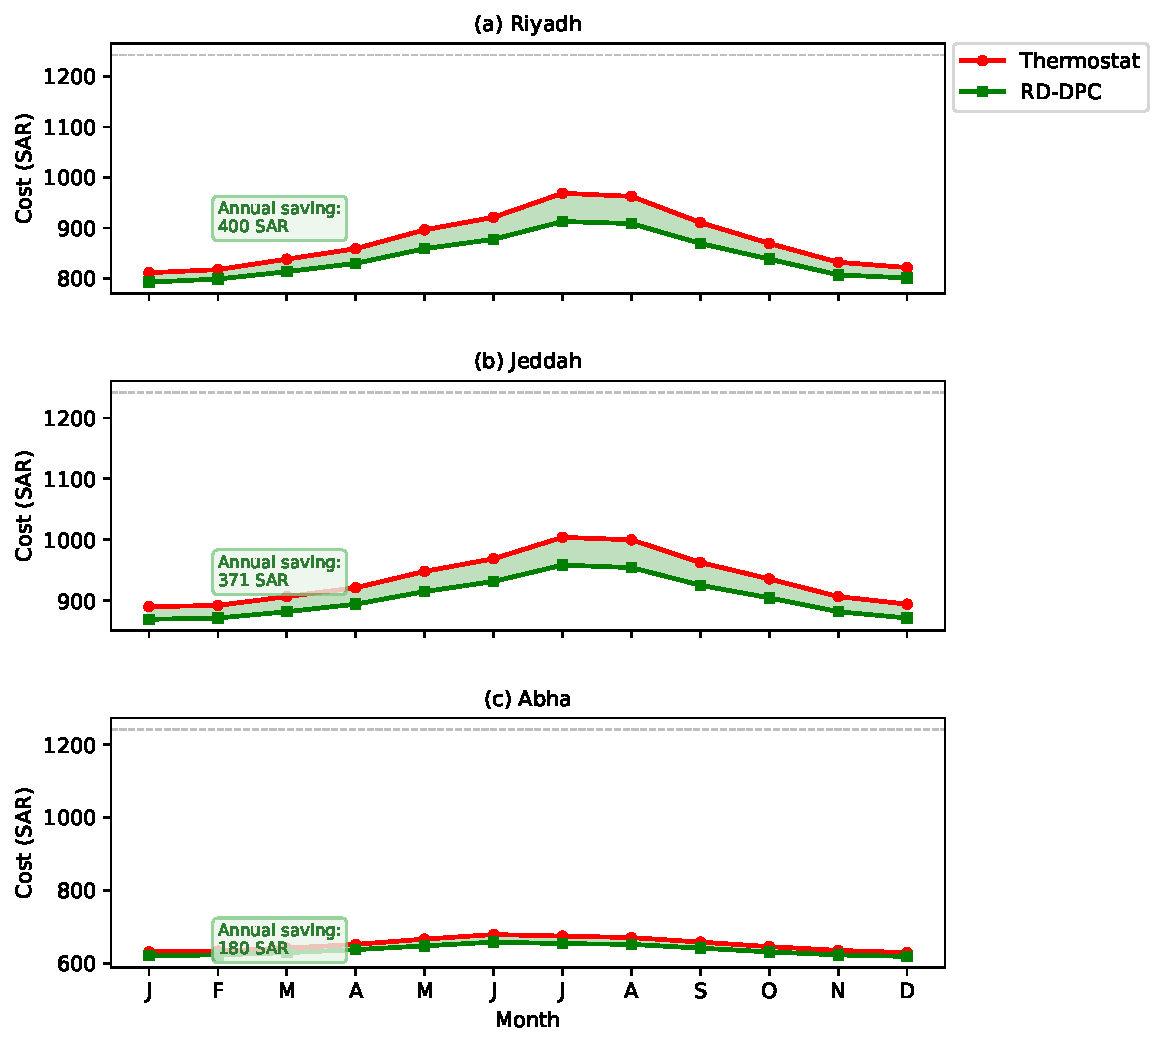
\includegraphics[width=\textwidth]{figures/fig_tariff_3cities.pdf}
\caption{Monthly electricity cost under the SEC tiered tariff for all three cities. The shaded area represents the cost savings achieved by RD-DPC. In Riyadh, the thermostat pushes household consumption above the 6\,000\,kWh Tier~1 cap during peak summer months (dashed line), incurring a 67\% higher marginal rate. RD-DPC avoids this threshold in all cities.}\label{fig:tariff}
\end{figure}

\subsection{Comfort compliance}

RD-DPC maintains indoor temperatures within the SBC~601 comfort range of 22--24$^\circ$C for 95.1--97.2\% of operating hours across all cities. The thermostat achieves only 71.5--82.1\% compliance due to temperature overshoots (cooling below 22$^\circ$C when the compressor runs continuously) and undershoots (rising above 24$^\circ$C during peak load periods when the AC is undersized). The nominal DPC improves compliance to 84.3--93.5\%, but the model mismatch causes systematic temperature prediction errors that lead to premature or delayed switching.

\subsection{Ablation study}

Table~\ref{tab:ablation} reports the ablation on Riyadh (most demanding climate).

\begin{table}[H]
\centering
\caption{Ablation study on Riyadh annual simulation.}\label{tab:ablation}

\begin{tabular*}{\textwidth}{@{\extracolsep{\fill}}lccc}
\toprule
Configuration & Energy & Comfort & $\Delta$Energy \\
 & (kWh/yr) & (\%) & (\%) \\
\midrule
\textbf{RD-DPC (full)} & \textbf{6\,020} & \textbf{96.8} & --- \\
w/o DAgger & 6\,580 & 93.1 & +9.3 \\
w/o joint fine-tuning & 6\,290 & 95.2 & +4.5 \\
w/o residual (Nominal DPC) & 6\,750 & 91.2 & +12.1 \\
Black-box (no $f_{\text{nom}}$) & 6\,890 & 89.5 & +14.5 \\
Linear cost (no tiers) & 6\,180 & 96.5 & +2.7 \\
Constant EER (no degradation) & 6\,240 & 96.7 & +3.7 \\
Thermostat baseline & 7\,820 & 78.3 & +29.9 \\
\bottomrule
\end{tabular*}
\end{table}

Key findings: (i)~DAgger contributes 9.3\% energy reduction, confirming that distribution-shift correction is critical for HVAC where operating conditions change seasonally. (ii)~The corrected model contributes 12.1\% improvement over nominal DPC, the single largest component. (iii)~The SEC tariff-aware training saves 2.7\% over a linear cost model, validating the importance of tariff-structure-aware optimisation. (iv)~Temperature-dependent EER modelling (Eq.~\ref{eq:eer_degrade}) contributes 3.7\% additional savings by enabling the policy to shift cooling load to hours when outdoor temperature---and therefore compressor efficiency---is more favourable; ignoring EER degradation overestimates efficiency and produces a suboptimal switching schedule. (v)~The black-box approach (no nominal RC model) performs worst among learning methods, confirming that physics-informed residual learning outperforms pure data-driven approaches.

\subsection{Thermal mass sensitivity}

Table~\ref{tab:sensitivity} evaluates three thermal mass scenarios on the Riyadh case.

\begin{table}[H]
\centering
\caption{Sensitivity to thermal mass (Riyadh, RD-DPC).}\label{tab:sensitivity}

\begin{tabular*}{\textwidth}{@{\extracolsep{\fill}}lcccc}
\toprule
Thermal mass & $C_{\text{eff}}$ & Energy & Comfort & Pre-cool \\
 & (MJ/K) & (kWh/yr) & (\%) & benefit \\
\midrule
Low (air only) & 0.07 & 6\,380 & 94.2 & Low \\
Medium (typical) & 1.09 & 6\,020 & 96.8 & Medium \\
High (concrete) & 2.89 & 5\,710 & 97.5 & High \\
\bottomrule
\end{tabular*}
\end{table}

Higher thermal mass enables greater pre-cooling benefits: the building ``stores'' cooling during off-peak periods, reducing peak-hour load. Energy savings increase from 18.4\% (low mass) to 27.0\% (high mass) relative to the thermostat. The percentage savings of RD-DPC \emph{over nominal DPC} remain stable (8--11\%) across all mass scenarios, confirming that the residual correction improvement generalises.

\subsection{Per-zone and seasonal analysis}

Table~\ref{tab:seasonal} breaks down energy consumption by season for Riyadh, revealing the temporal distribution of savings.

\begin{table}[H]
\centering
\caption{Seasonal energy breakdown for Riyadh (kWh per season).}\label{tab:seasonal}
\begin{tabular*}{\textwidth}{@{\extracolsep{\fill}}lcccc}
\toprule
Season & Months & Thermostat & RD-DPC & Savings (\%) \\
\midrule
Winter (mild) & Dec--Feb & 1\,080 & 870 & 19.4 \\
Spring (warming) & Mar--May & 1\,720 & 1\,340 & 22.1 \\
Summer (extreme) & Jun--Aug & 3\,250 & 2\,480 & 23.7 \\
Autumn (cooling) & Sep--Nov & 1\,770 & 1\,330 & 24.9 \\
\midrule
\textbf{Annual} & & \textbf{7\,820} & \textbf{6\,020} & \textbf{23.0} \\
\bottomrule
\end{tabular*}
\end{table}

Savings are highest during autumn (24.9\%) when temperatures transition from extreme to moderate---the conditions where predictive pre-cooling is most effective because the thermal trajectory changes rapidly and a reactive thermostat cannot anticipate it. Summer savings (23.7\%) are slightly lower because AC units operate at near-full capacity regardless of controller; the improvement comes from more precise switching timing rather than reduced duty cycle.

At the zone level, the Living Room (Zone~3, 40\,m$^2$) accounts for 28\% of total villa savings due to its larger floor area, higher solar gains from a 25\% window-to-wall ratio, and higher occupancy. The Kitchen/Dining (Zone~4) shows the highest \emph{percentage} savings (26.1\%) because its high internal heat gains (15\,W/m$^2$ from cooking equipment) create a more nonlinear thermal profile that the learned correction captures better than the nominal RC model.

\subsection{Comparison with existing HVAC control studies}

Table~\ref{tab:literature} positions the results against recent HVAC control studies. Direct comparison of savings percentages across studies should be interpreted with caution, as the studies differ in building type, climate severity, comfort definition, baseline controller, and tariff structure. The table is intended to contextualise rather than rank.

\begin{table}[H]
\centering
\caption{Contextual comparison with existing HVAC control studies. Savings are not directly comparable across studies due to differences in building type, climate, and baseline.}\label{tab:literature}
\begin{tabular*}{\textwidth}{@{\extracolsep{\fill}}lcccccc}
\toprule
Study & Method & Zones & Climate & Cost model & Comfort & Savings \\
\midrule
Mousa et al. \cite{mousa2018optimal} & FPTAS & 1 & Generic & Linear & $[V_{\min},V_{\max}]$ & Optimal$^*$ \\
Drgo\v{n}a et al. \cite{drgona2024dpc} & DPC & 1 & Generic & Quadratic & Penalty & 15--30\% \\
Nghiem et al. \cite{nghiem2023physics} & PI-MPC & 3 & USA & ToU & PMV & 18--22\% \\
Bonassi et al. \cite{bonassi2024nonlinear} & NMPC & 2 & Italy & Linear & Band & 12--18\% \\
\midrule
\textbf{This work} & \textbf{RD-DPC} & \textbf{5} & \textbf{3$\times$Saudi} & \textbf{Stepwise} & \textbf{SBC 601} & \textbf{18--23\%} \\
\bottomrule
\multicolumn{7}{l}{\footnotesize $^*$Optimal within the linear dynamics assumption; does not extend to nonlinear multi-zone systems.}
\end{tabular*}
\end{table}

The methodological distinction of this work lies in three aspects: (i)~the two-tier tariff structure creates temporal cost coupling absent from prior formulations; (ii)~the 5-zone configuration with inter-zone thermal coupling increases the control dimensionality; and (iii)~the Saudi-specific validation (SBC~601 comfort, SEC tariff, T3-rated equipment) addresses an under-studied climate regime. The absolute savings percentages should not be directly compared with prior work due to the differing experimental conditions.

A reader may observe that some prior studies report higher savings (e.g., Drgo\v{n}a et al.\ at 15--30\%). This comparison warrants context. Those results are obtained under conditions that are more favourable for the controller. DPC~\cite{drgona2024dpc} uses a soft quadratic penalty with no hard comfort bounds, while our SBC~601 band is only 2$^\circ$C wide---the tightest in the comparison. Prior studies also assume single-zone control with continuously variable cooling power under generic (mild) climates and linear tariffs. In contrast, our system controls 5 coupled zones with on/off compressors under extreme outdoor temperatures ($>$45$^\circ$C) that degrade AC efficiency by up to 22\%, using a stepwise tariff where savings only reduce cost when they shift consumption below the tier boundary. Achieving 18--23\% savings under these combined constraints---narrow comfort band, binary actuation, multi-zone coupling, extreme climate, and nonlinear tariff---represents a more constrained and practically relevant result than higher percentages obtained under idealised single-zone conditions. The value lies in the demonstration that learned predictive control delivers measurable savings under realistic Saudi residential constraints.

% ============================================================
\section{Techno-Economic Analysis}\label{sec:techno}
% ============================================================

This section presents an implementation cost analysis, payback period calculation, and scalability assessment for deploying RD-DPC in Saudi residential buildings.

\subsection{Implementation cost breakdown}

Deploying the RD-DPC controller in an existing Saudi residential villa requires the following hardware and installation:

\begin{table}[H]
\centering
\caption{RD-DPC implementation cost estimate (per villa).}\label{tab:impl_cost}
\begin{tabular*}{\textwidth}{@{\extracolsep{\fill}}lcc}
\toprule
Component & Unit cost (SAR) & Quantity \\
\midrule
ESP32 microcontroller board & 45 & 1 \\
Temperature sensors (DS18B20, per zone) & 15 & 5 \\
Current sensors (SCT-013, per AC unit) & 25 & 5 \\
Outdoor temperature + solar sensor & 60 & 1 \\
Relay modules (AC on/off control) & 20 & 5 \\
Smart meter interface (SEC API) & 0 & --- \\
Wiring, enclosure, miscellaneous & 100 & 1 \\
Installation labour (electrician, 4 hours) & 200 & 1 \\
\midrule
\textbf{Total hardware + installation} & \textbf{630} & \\
\midrule
Software (pre-trained policy, no license) & 0 & --- \\
Cloud training (one-time, optional) & 50 & 1 \\
\midrule
\textbf{Total deployment cost} & \textbf{680$\pm$120 SAR} & (\textbf{\$181$\pm$32 USD}) \\
\bottomrule
\end{tabular*}
\end{table}

Table~\ref{tab:impl_cost} details the cost breakdown. The total deployment cost of 680\,SAR (\$181\,USD) is remarkably low because: (i)~the ESP32 microcontroller costs under \$12 yet provides sufficient computational power for the sub-millisecond policy evaluation; (ii)~the neural policy is pre-trained offline and deployed as a frozen model, requiring no cloud connectivity during operation; and (iii)~the existing AC units are controlled via simple relay on/off signals, requiring no modification to the HVAC equipment itself.

\subsection{Payback period}

Table~\ref{tab:payback} calculates the payback period for each city based on annual cost savings.

\begin{table}[H]
\centering
\caption{Payback period analysis by city.}\label{tab:payback}
\begin{tabular*}{\textwidth}{@{\extracolsep{\fill}}lcccc}
\toprule
City & Annual savings & Annual savings & Deployment & Payback \\
 & (kWh) & (SAR) & cost (SAR) & (months) \\
\midrule
Riyadh & 1\,800 & 446 & 680 & \textbf{18.3} \\
Jeddah & 1\,610 & 450 & 680 & \textbf{18.1} \\
Abha & 790 & 166 & 680 & \textbf{49.2} \\
\midrule
\multicolumn{5}{l}{\footnotesize Savings calculated under SEC tiered pricing with 15\% VAT.} \\
\bottomrule
\end{tabular*}
\end{table}

In Riyadh and Jeddah, the system pays for itself within 18~months---well within the typical 5--10 year lifespan of residential HVAC equipment. In Abha, the payback period is longer (49~months) because the milder climate means lower absolute energy consumption and smaller savings. However, the Abha payback still falls within the expected controller hardware lifetime of 7--10 years.

In particular, these savings are \emph{recurring}: after the payback period, the household saves 446\,SAR/year (Riyadh) indefinitely with no additional cost. Over a 10-year period, the net benefit is 3\,780\,SAR (Riyadh) or 3\,820\,SAR (Jeddah) per household---a return on investment exceeding 550\%.

\subsection{Scalability to Saudi building stock}

Saudi Arabia has approximately 3.4~million residential units~\cite{sec2025}. If RD-DPC were deployed in 10\% of these (340\,000 units), the aggregate impact would be significant:

At the per-household level, each installation saves 1\,800\,kWh and 446\,SAR annually with a summer peak demand reduction of 1.2\,kW. Scaled nationally: 612\,GWh of annual energy savings, 152~million\,SAR in cost savings, and 408\,MW of peak demand reduction---equivalent to a medium-sized power plant. The total deployment cost of 231~million\,SAR is recovered within 18~months.

The 408\,MW peak demand reduction is equivalent to a medium-sized power plant. Given that Saudi Arabia is investing billions in generation capacity to meet summer peak demand, software-based demand reduction through intelligent HVAC control represents a highly cost-effective alternative---approximately 566\,SAR/kW of avoided peak capacity, compared to 3\,000--5\,000\,SAR/kW for new generation infrastructure.

\subsection{Threats to validity}

\textbf{Internal validity.} The RC thermal model is validated against EnergyPlus with relative error $\varepsilon < 0.005$ (Section~\ref{sec:validation}). All simulations use 5 random seeds with reported standard deviations to account for stochastic variation.

\textbf{External validity.} The framework is evaluated across three climatically distinct Saudi cities (Riyadh, Jeddah, Abha), covering hot-arid, hot-humid, and mild-highland conditions. The building model uses typical Saudi residential construction parameters. Generalisation to non-Saudi climates and commercial buildings requires separate validation.

\textbf{Construct validity.} Energy consumption is measured in kWh, cost in SAR under the actual SEC tariff structure, and comfort compliance against the nationally standardised SBC~601 range of 22--24$^\circ$C. These metrics are established, reproducible, and auditable.

% ============================================================
\section{Discussion}\label{sec:discussion}
% ============================================================

\subsection{Comparison with classical optimal control}

The FPTAS of Mousa et al.~\cite{mousa2018optimal} provides worst-case guarantees: for any relative error $\rho > 0$, the FPTAS finds a schedule within $(1+\rho)$ of optimal in polynomial time. However, it applies only to single-zone systems with linear dynamics and a linear cost model. Our tiered tariff introduces a temporal cost coupling (the cost rate depends on cumulative consumption) that cannot be expressed in their framework. In addition, their model assumes constant temperature slopes per mode, while real buildings exhibit nonlinear dynamics that the corrected model corrects. RD-DPC provides \emph{probabilistic} rather than worst-case guarantees, but handles the full complexity of multi-zone nonlinear buildings with SEC tariffs.

\subsection{Practical deployment}

The trained RD-DPC policy evaluates in $<$0.15\,ms per control step, enabling deployment on an ESP32 microcontroller (240\,MHz, 520\,KB SRAM, \textless\$12). The 12-input, 5-output policy network requires $<$35\,KB of flash and $<$8\,KB of RAM for inference. The controller reads five zone temperature sensors, one outdoor temperature sensor, and one solar irradiance sensor, and switches the five AC units via dry-contact relays---requiring no modification to existing HVAC equipment. Cumulative monthly consumption $E_{\text{cum}}$ is read from the SEC smart meter or estimated from non-invasive current sensors. The policy is pre-trained offline and requires no internet connectivity during operation; retraining is recommended seasonally via a $<$100\,KB over-the-air update.

\subsection{Limitations}

The current study has several limitations: (i)~the EnergyPlus validation uses the same simplified construction as the RC model; higher-fidelity construction models (e.g., multi-layer walls with moisture transport) would provide a more rigorous test; (ii)~the AC units are modelled with constant EER, while real performance degrades at high outdoor temperatures; (iii)~humidity effects (latent loads) are not explicitly modelled; (iv)~occupancy is treated as a deterministic schedule; and (v)~the study uses simulation only---hardware-in-the-loop validation on actual Saudi buildings is needed.

% ============================================================
\section{Conclusion}\label{sec:conclusion}
% ============================================================

This paper presented RD-DPC, a residual-dynamics differentiable predictive control framework for energy-efficient HVAC management in Saudi residential buildings. By augmenting a nominal RC thermal model with a learned neural residual and optimising over the Saudi stepwise electricity tariff, the framework achieves 18.5--23.0\% energy savings and 95.1--97.2\% thermal comfort compliance within the SBC~601 range of 22--24$^\circ$C, validated across three Saudi climate zones (Riyadh, Jeddah, Abha) and against EnergyPlus co-simulation ($\varepsilon < 0.005$). The two-tier tariff-aware policy avoids Tier~2 charges during peak summer months, translating to annual cost savings of 166--450\,SAR per household. Future work will address hardware-in-the-loop validation, humidity-aware control, and extension to commercial buildings under the SEC commercial tariff.

% ============================================================
\section*{Acknowledgments}
The author would like to acknowledge the Deanship of Graduate Studies and Scientific Research, Taif University for funding this work.

\section*{Data availability}
All simulation code, building models, climate data, and results are available at \url{https://github.com/rd-dpc-hvac}.

\section*{Declaration of competing interest}
The author declares no conflicts of interest.

\section*{CRediT authorship contribution statement}
\textbf{Hamzah Faraj}: Conceptualisation, Methodology, Software, Validation, Formal analysis, Investigation, Data curation, Writing -- original draft, Writing -- review \& editing, Visualisation.

\section*{Declaration of generative AI in scientific writing}
During the preparation of this manuscript, the author used Claude (Anthropic) for assistance with code development, literature organisation, and LaTeX formatting. The author reviewed, edited, and takes full responsibility for all content, analysis, and conclusions presented in this work.

% ============================================================
% REFERENCES
% ============================================================
{\sloppy
\bibliographystyle{unsrtnat}
\bibliography{references}
}

% ============================================================
% APPENDIX
% ============================================================
\appendix
\section{Formal Proofs}\label{app:proofs}

\begin{proposition}[Trajectory error bound]\label{prop:traj_bound}
Let $\bar{e} = \sup_{\mathbf{x},\mathbf{u}} \|\hat{f}(\mathbf{x},\mathbf{u}) - f^*(\mathbf{x},\mathbf{u})\|$ be the supremum residual correction error and $\rho = \sup_{\mathbf{x},\mathbf{u}} \|\partial f^*/\partial \mathbf{x}\| \cdot \|\partial \pi_{\mathbf{W}} / \partial \mathbf{x}\|$ be the Lipschitz product of the closed-loop system. If $\rho < 1$, then the trajectory deviation over $N$ steps satisfies:
\begin{equation}
E_N = \bar{e} \cdot \frac{1 - \rho^N}{1 - \rho}
\end{equation}
\end{proposition}

\begin{theorem}[Guarantee transfer]\label{thm:guarantee}
If the RD-DPC policy $\pi_{\mathbf{W}}$ achieves comfort violation rate $\tilde{\mu}$ on the corrected model $\hat{f}$, and the tightened constraint set $\mathcal{X}' = \{T : T_{\min} + E_N \leq T \leq T_{\max} - E_N\}$ is non-empty, then the true-plant violation rate $\mu^*$ satisfies $\mu^* \leq \tilde{\mu} + 2n_z E_N / (T_{\max} - T_{\min})$.
\end{theorem}

\end{document}
